\documentclass[border=10pt]{standalone}
\usepackage[svgnames]{xcolor}
\usepackage{amsmath}
\usepackage{pgfplots}
\pgfplotsset{compat=newest}
\usepackage[sfdefault]{FiraSans}
\usepackage{FiraMono}
\renewcommand*\familydefault{\sfdefault}
\begin{document}
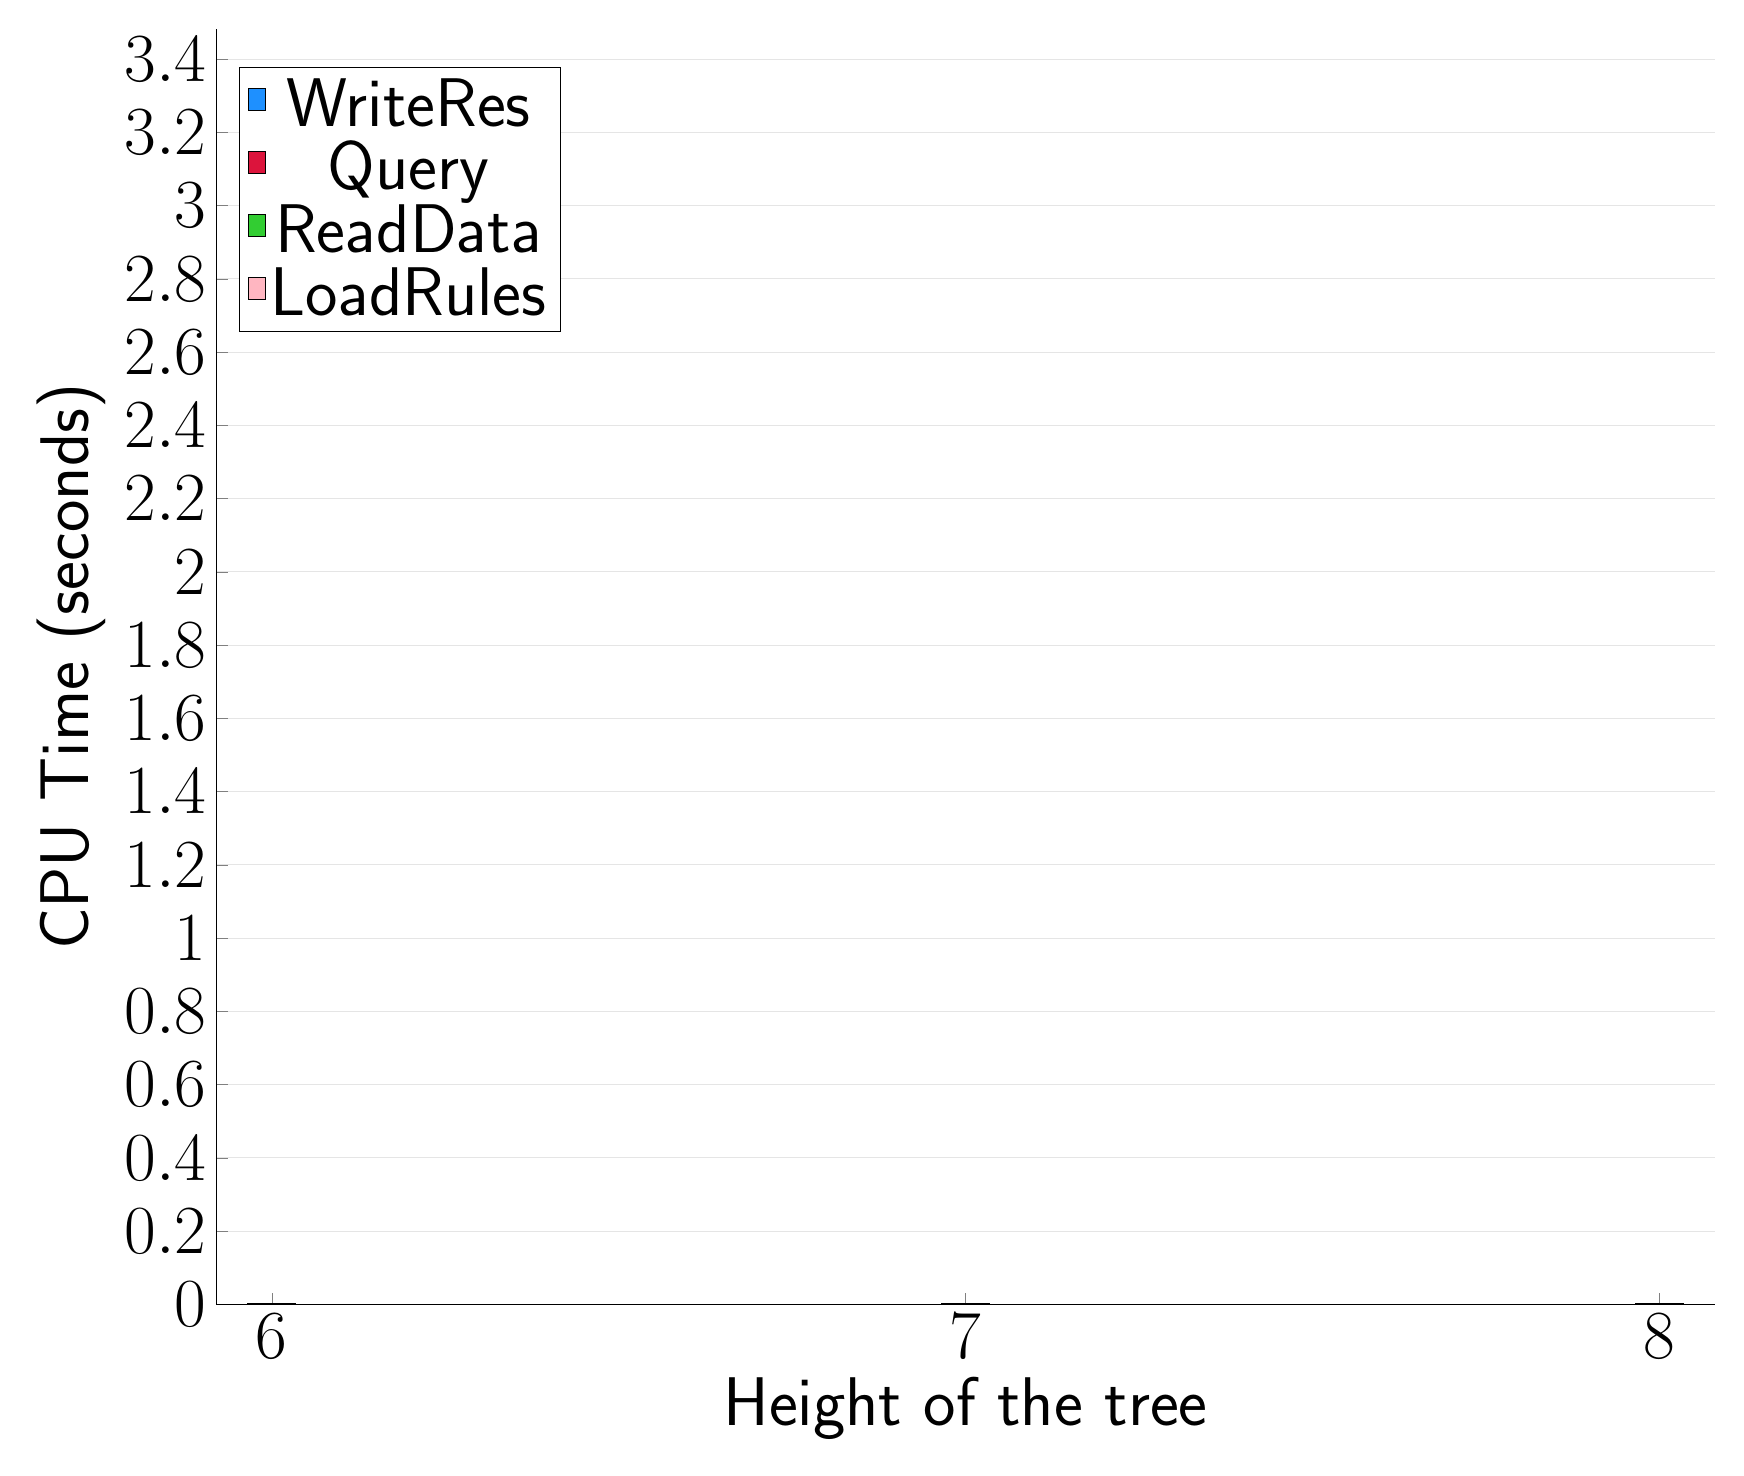
\begin{tikzpicture}
\begin{axis}[
   ybar stacked,
   width=1.7\textwidth,
   bar width=0.6cm,
   ymajorgrids, tick align=inside,
   major grid style={draw=gray!20},
   xtick=data,
   ymin=0, ymax=3.4819999999999998,
   axis x line*=bottom,
   axis y line*=left,
   enlarge x limits=0.04,
   legend style={
       at={(0.23, 0.97)},
       anchor=north east,
       legend columns=1,
       font=\Huge,
   },
   ylabel={CPU Time (seconds)},
   xlabel={Height of the tree},
   label style={font=\Huge},
   tick label style={font=\Huge},
]
\addlegendimage{fill=DodgerBlue, draw=black, line width=0.2pt}
\addlegendentry{WriteRes}
\addlegendimage{fill=Crimson, draw=black, line width=0.2pt}
\addlegendentry{Query}
\addlegendimage{fill=LimeGreen, draw=black, line width=0.2pt}
\addlegendentry{ReadData}
\addlegendimage{fill=LightPink, draw=black, line width=0.2pt}
\addlegendentry{LoadRules}
\addplot +[fill=LightPink, draw=black, line width=0.55pt] coordinates {
(6, 0.0005598000000000003)
(7, 0.0005499999999999995)
(8, 0.0005478000000000006)
(8, 0.0005494000000000002)
};
\addplot +[fill=LimeGreen, draw=black, line width=0.55pt] coordinates {
(6, 0.00016739999999999979)
(7, 0.00021979999999999976)
(8, 0.0003181999999999998)
(8, 0.00031959999999999996)
};
\addplot +[fill=Crimson, draw=black, line width=0.55pt] coordinates {
(6, 3.82000000000004e-05)
(7, 7.659999999999994e-05)
(8, 0.0001729999999999996)
(8, 0.00017299999999999981)
};
\addplot +[fill=DodgerBlue, draw=black, line width=0.55pt] coordinates {
(6, 0.0002678)
(7, 0.0005840000000000002)
(8, 0.0013202000000000005)
(8, 0.0013190000000000003)
};
\end{axis}
\end{tikzpicture}

\end{document}
